\documentclass{article}
\usepackage{color}
\usepackage{cite}
\usepackage{hyperref}
\usepackage{graphicx}
\usepackage{siunitx}
\usepackage{placeins}
\usepackage{longtable}
\newcommand{\hl}[1]
{\colorbox{yellow}{#1}}
\title{Making Secure Easy-to-Remember Passwords}
\author{Philip Braunstein}
\date{December 14, 2015}
\begin{document}

\maketitle
\abstract{
Password leaks are a notorious way that systems get compromised. Passwords are often leaked exactly because they are heard to remember, which prompts people to record them in insecure locations and avoid changing them. This report describes and evaluates three password generation strategies. Three password generation strategies are evaluated in this report: random strings of characters, numbers, and symbols (RS); abbreviations of phrases mixed with meaningful numbers (MPM); and an adjective-noun-verb-adjective-noun string modeled after xkcd 936 (MX) \hl{SOURCE: XKCD}. Passwords were evaluated on ease of memorization, cryptographic strength against a password cracker, and bits of entropy. MPM passwords were easiest to remember by woefully insecure in terms of entropy per password as well as vulnerability to a password cracker. MX passwords had by leaps and bounds the highest entropy per password of any password type. MX passwords were easy for participants to remember, and participants made quick learning gains when MX passwords were incorrectly remembered.
}

\section*{Introduction}
People like to imagine that computer security is usually compromised by genius hackers exploiting inscrutable vulnerabilities. Often however, an attacker compromises a system because of seemingly stupid reasons like the being written on a note next to the computer. Shoring up technical security is a worthy cause, but this effort is rendered irrelevant unless the impact of social engineering resulting in password leaks is minimized. 

People avoid changing their passwords, leave them written in plain text in a document on their computer or even on a sticky note on their computer for one reason only: secure passwords are hard to remember. Insecure and poorly-stored passwords are the cause of many security leaks \hl{FIND SOME GENERAL SOURCES}. Passwords are a common source of vulnerability because different websites have different requirements for what they consider valid passwords, and passwords that are considered secure are obtuse and hard for people to remember.

In this report, three methods for making passwords are described and evaluated. The security and how easy each type of password to remember is evaluated and described in the Results section.

\section*{To the Community}
I am particularly interested in passwords because passwords are an intersection of humans and computers. Humans and computers have varying strengths and weaknesses, which makes choosing the right passwords tricky. Passwords need to be secure enough so they don't get easily cracked with a tool like Hashcat, but they also need to be possible for people to remember. Passwords that are too simple get cracked by a program such as Hashcat, and passwords that are too complicated get hacked because people leave them written in obvious places or never change them.

\section*{Methods}
\subsection*{Overall Description of Procedure}
Each of the password generation methods described below were tested on a total of 7 subjects. In order to prevent bias based on subjects getting used to the memorization task, the script \texttt{determineOrder.py} was used to dictate the order that each of the password methods was tested. For the random string and modified XKCD password style, participants were shown 10 options for passwords and were permitted to chose the preferred password. Participants were told there were no length requirements for the MPM password, and they were not informed of the length of the RS and MX passwords.

For each password method, participants chose the password they wanted to use, and participants were not permitted to write the password down. Participants were then instructed to focus on something else. Most went back to work, and some chatted with me during that time. When I was speaking with a participant, I tried to steer the conversation away from the topic of the password that they chose. After five minutes, participants were asked to write their password down. If they wrote the password down exactly correctly, they were informed that they remembered their password perfectly. If they messed up their password, they were either told what was amiss with their guess (e.g. ``the correct password is \texttt{casualpiebecomesonlyprofit} instead of \texttt{otherpiebecomesonlyprofit} or they were shown the correct password for another couple of seconds. Participants worked or chatted with me for another five minutes, and then wrote down their passwords again. Passwords were tested one at a time. It was at no time during the experiment necessary for participants to remember more than one password. As an example, Participant 1 first only had to remember the random string password, then only the modified XKCD password, and then only the memorable phrase and number password.

Learning gains were evaluated for each password type as follows: for each password type, the similarity of the first trial was subtracted from the similarity of the password trial. However, only those passwords, in which the first trial similarities were less than 1 were counted. 

Error bars were not included for any of the figures in the experiment because 7 participants is not a large enough sample size. In order to get estimates on error, a larger study should be conducted.



\subsection*{Password Generation Schemes}
\subsubsection*{Random String}
A random string password consists of ten random characters, numbers, and symbols. A random string passwords must have contain at least one of three of the four categories: upper-case letter, lower-case letter, number, or symbol. The script \texttt{randomPass.py} generates ten of these random strings passwords. Participants selected one of the ten passwords to use.


\subsubsection*{Memorable Phrase and Number}
Participants chose a memorable phrase and made an acronym of the first letter of each word. Every initial was lower-case in the password. They also chose a particular number and incorporated it after the initials of the memorable phrase. For example, I might choose the hook from a famous Rolling Stones song (\textbf{I} \textbf{c}an't \textbf{g}et \textbf{n}o \textbf{s}atisfaction, and the month and year of my graduation from college (May, 2012) to generate the following password: icgns0512. 

\subsubsection*{Modified XKCD}
Randall Munroe of XKCD suggests using several common words that can be used to create a more coherent memory as opposed to other password generation methods. I have improved on his idea by forcing passwords to obey the form adjective noun verb adjective noun, where the words from these parts of speech are drawn from publicly available word lists \hl{CITE WORD LISTS}.

The script \texttt{humanPass.py} creates ten of these modified XKCD passwords, from which the participant chose one. The passwords were written with all lower case letters and no spaces between the words. Participants were allowed to alter the password to fix any grammatical mistakes. For example one password generated by \texttt{humanPass.py} was \texttt{availablenervebitemolecularradish} (available nerve bite molecular radish). Participants were instructed to modify the passwords so that they make grammatical sense, but the exact modification was left to the discretion of the participant. For example, the previous password could be modified in one of two ways \texttt{availablenervebitesmolecularradish} (available nerve bites molecular radish) or \texttt{availablenervesbitemolecularradish} (available nerves bite molecular radish). Participants were encouraged to make whatever grammatical modification makes the most sense to them.

\subsection*{Password Evaluation}
The passwords were evaluated on three criteria: the success of a participant remembering the password, the strength of the password against password cracking, and the number of bits of entropy.
\subsubsection*{Success Remembering Password}
At first glance, the success of a participant remembering a password should be measured by the percent similarity of the remembered password and the actual password. This could be calculated by comparing each character in the two passwords to see how similar they are. This method, however, is insufficient. Consider the following example:\\


\noindent\texttt{0123456789}\\
\texttt{023456789} \\

These two passwords result in a similarity of 0.1 since the `1' is omitted in the second password. However, nine of ten of the characters were successfully remembered. Therefore, this simple metric of similarity under-represents how similar the two passwords actually are. In short, a simple percent similarity metric does not account for character insertions or deletions in the sequences.

To compensate for this problem, the script \texttt{smartFracSim.py} calculates the fraction similar of the two passwords from the forward direction \emph{and} from the reverse direction and averages these values (hereafter: smart fraction similar). This raises the fraction similar of the example to 0.45 $((0.1 + 0.8 / 2.0))$.

While the smart fraction similar is a better metric than fraction similar of only one direction, I still believed that this metric was under-representing the similarity in the passwords. Consider the modified xkcd example password from above: \\

\noindent \texttt{availablenervebitesmolecularradish} (available nerve bites molecular radish) \\

Consider what would happen if a participant swapped the adjectives to make the following password:\\

\noindent \texttt{molecularnervebitesavailableradish} (molecular nerve bites available radish). \\

The original and adjective-swapped passwords have a smart fraction similar of 0.47. This significantly under-represents the how close the participant was to correctly remembering the password. The participant simply flipped the adjectives, and might score a 1.0 similarity if asked again. In order to compensate for this, the modified XKCD passwords were also analyzed for similarity as follows: what fraction of the original words were also present in the remembered password, regardless of the grammatical form (for example, \texttt{nerve} would count when matched with \texttt{nerves}). This word similarity metric was averaged with the smart fraction similar metric to compute the final similarity for the modified XKCD passwords. In the swapped adjectives example, the word fraction similar is 1.0 (all words are present). Averaged with the smart fraction similar, the final similarity fraction for this example is 0.74. The word fraction was determined by hand (by me), since it would have been difficult to write a script to recognize the varying valid grammatical forms of word as well as where to break the password string into a word.

The word fraction similarity metric is successful because it accounts for distinct parts of the password that a participant has successfully remembered. There is no exact corresponding metric for the random string and memorable phrase and number passwords. So, the fraction of characters similar between the original password and remembered password was determined for these styles of password using the script \texttt{charFracSim.py}. As above, this metric is averaged with the smart fraction similar to calculate the final similarity for random string and memorable phrase and number passwords.


\subsubsection*{Strength Against Password Cracking}
The MD5 hash of the passwords was determined using built in Python hashing functionality with the script \texttt{makeHashes.py}. A distribution of Kali Linux running in a virtual machine on my Mac was used for the password cracking. 2 GB of RAM was allocated to the virtual machine. The mask attack of the program Hashcat was used for cracking the RS and the MPM passwords. The mask attack is a brute-force attack in which the user supplies a mask which describes the type of characters that should be attempted at each position where \%d signifies a digit, \%l signifies a lower-case letter, and \%a signifies all possible characters. The mask makes the brute-force attack more efficient and more targeted.

The complete invocation of Hashcat to attempt to break RS password hashes was: \\

\texttt{time /usr/bin/hashcat --hash 0 --attack-mode 3 --pw-min 10 hashes.txt \%a\%a\%a\%a\%a\%a\%a\%a\%a\%a} \\

where \texttt{--hash 0} indicates that MD5 without salt was used to has the passwords, \texttt{--attack-mode 3} indicates a mask attack should be used, \texttt{--pw-min} indicates the smallest length password guessed should be 10 (so Hashcat didn't increment through shorter length password guesses), \texttt{hashes.txt} is the file containing the hashes, and \texttt{\%a\%a\%a\%a\%a\%a\%a\%a\%a\%a} is the mask that indicates each of the 10 positions could be any character (equivalent to the deprecated brute-force attack). 

The MPM passwords have the predictable structure of a number of lower case letters followed by a couple of digits. Several runs of Hashcat with masks corresponding to the structure of every MPM password created by the participants of this study. The masks used were \texttt{\%l\%l\%l\%l\%d\%d}, \texttt{\%l\%l\%l\%l\%d\%d\%d\%d}, \texttt{\%l\%l\%l\%l\%l\%d\%d}, and \texttt{\%l\%l\%l\%l\%l\%d\%d\%d\%d}. The standard Unix function \texttt{time} was used to record the user time it took to run each cracking attempt.

Password cracking was not attempted to crack the hashes of the MX passwords because these passwords are far too long to be cracked with a mask attack. Calculations to approximate resistance to hacking attacks of the MX passwords is described in the results section.

\subsubsection*{Bits of Entropy}
The bits of entropy for each password was determined by calculating the number of possible passwords for a password of that style of that length. The entropy of the RS passwords ($H_{RS}$) was determined by the following formula:

$$H_{RS} = 94^{10}$$

in which there were 94 possibilities for each character and the overall length of the password was 10 characters. The 94 possibilities came from the following Python statement: \\

\texttt{len(strings.punctuation + strings.digits + strings.letters)}

The entropy of a MPM password $p$ ($H_{MPM}(p)$)was determined as follows:

$$H_{MPM}(p) = 26^l10^d$$

where $l$ is the number of lowercase letters in the MPM password and $d$ is the number of digits in the password.

The entropy of a MX password $p$ ($H_{MX}(p)$) was determined as follows:

$$H_{MX}(p) = 26^{len(p)}$$

MX passwords only contained lowercase letters, which is the derivation of the 26 possibilities per character.

\FloatBarrier
\section*{Results}
\subsection*{MPM are Easiest to Remember}
Of the 7 participants tested in the experiment, every single one of them remembered their MPM passwords for both trials of the experiment. MX passwords were remembered perfectly for every participant's second time being asked. A clear hierarchy of how easy each style password to remember emerges from these experiments: MPM passwords are the easiest to remember followed shortly by MX passwords, but the RS passwords are much harder to remember (Table 1 and Figure 1). Notice that RS passwords are clearly much more difficult to remember than either MPM or MX passwords (Figure 1).
\begin{figure}
\centering
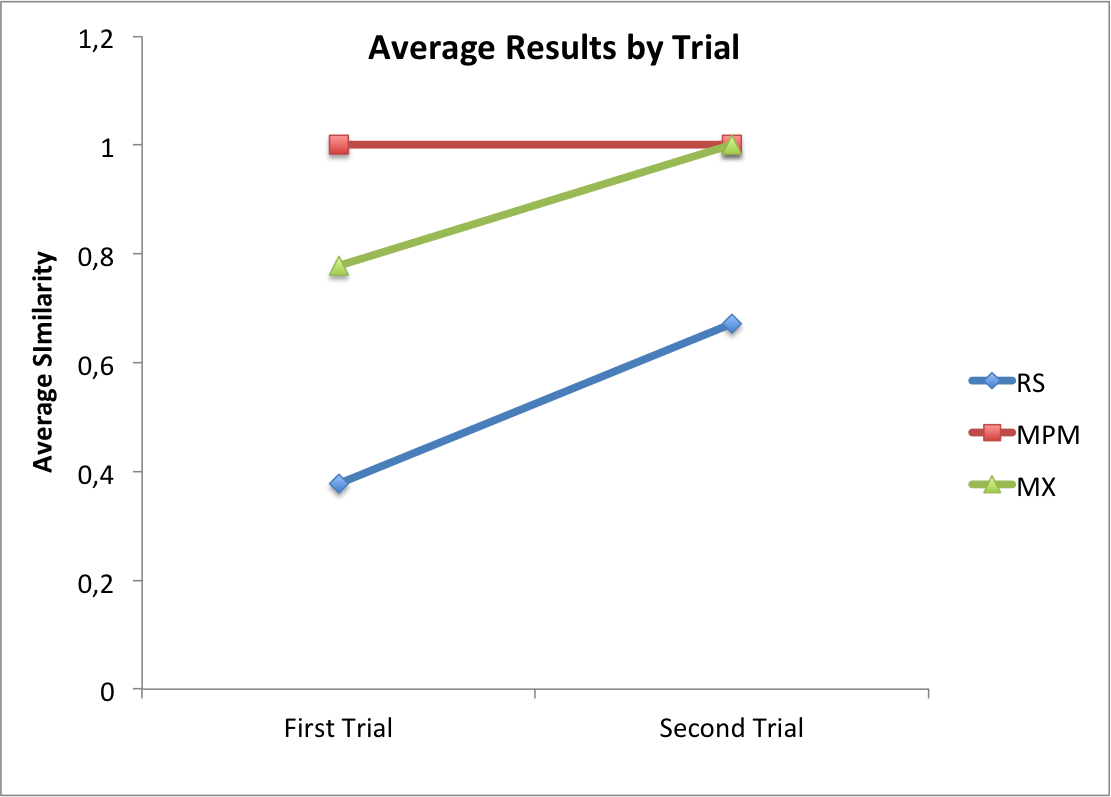
\includegraphics[scale=0.75]{resultsByTrial.png}
\caption{Average similarity by trial and password type}
\end{figure}

\begin{table}
\centering
\begin{tabular}{|c|c|c|}
\hline
Password Type & First Trial & Second Trial \\
\hline
RS & 0.34 & 0.67 \\
\hline
MPM & 1.0 & 1.0 \\
\hline
MX & 0.78 & 1.0 \\
\hline
\end{tabular}
\caption{Average similarity by trial and password type}
\end{table}

\subsection*{MX Passwords are Easier to Learn than RS Passwords}
Figure 2 shows that of the passwords that required learning (i.e. the participant did not remember the password entirely correctly the first time asked), MX passwords are easier to learn than the RS passwords. 
\begin{figure}[h]
\centering
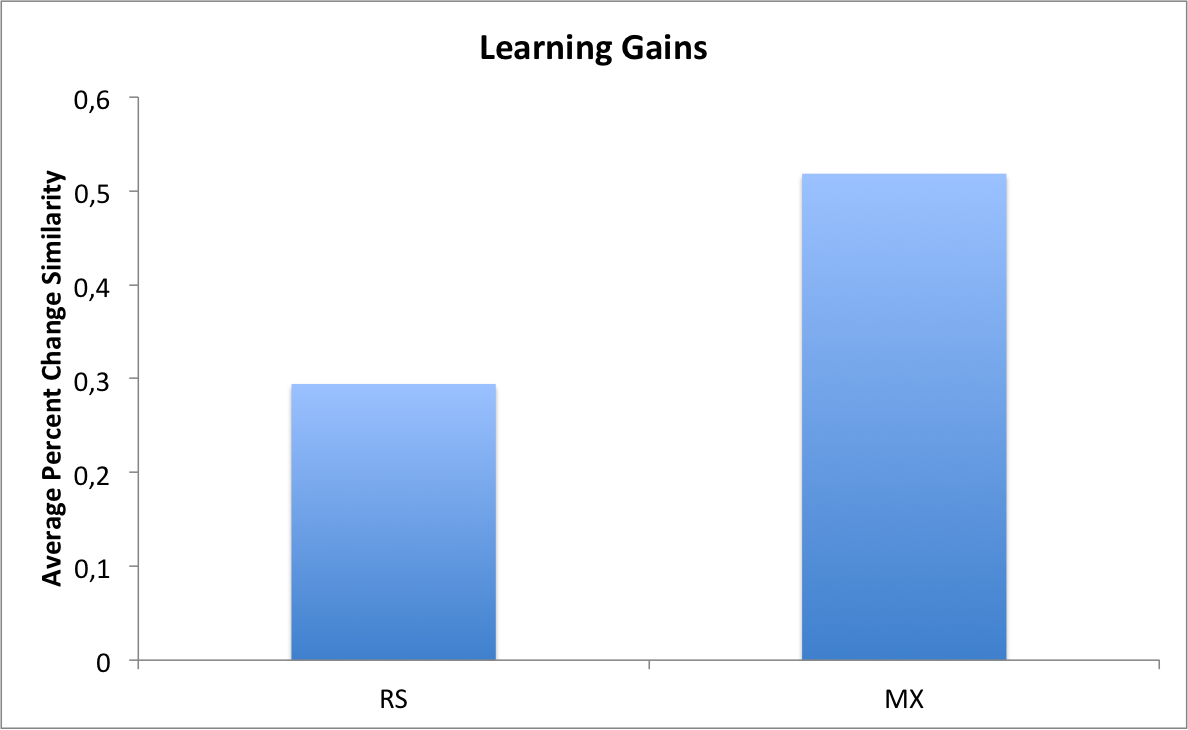
\includegraphics[scale=0.7]{learningGains.png}
\caption{Learning gains for RS and MX}
\end{figure}

\subsection*{MX Passwords Have by Far the Highest Entropy}
The average  entropy and average $log_{10}$ entropy for each password style is displayed in Table 2. Figure 3 and Table 3 shows the incredible gains of entropy seen by using MX passwords. MX passwords have on average \num{1.1e36} times more entropy than RS passwords, and MX passwords have on average \num{1.2e44} times more entropy than MPM passwords. MPM passwords had the lowest entropy. 

\begin{figure}[h]
\centering
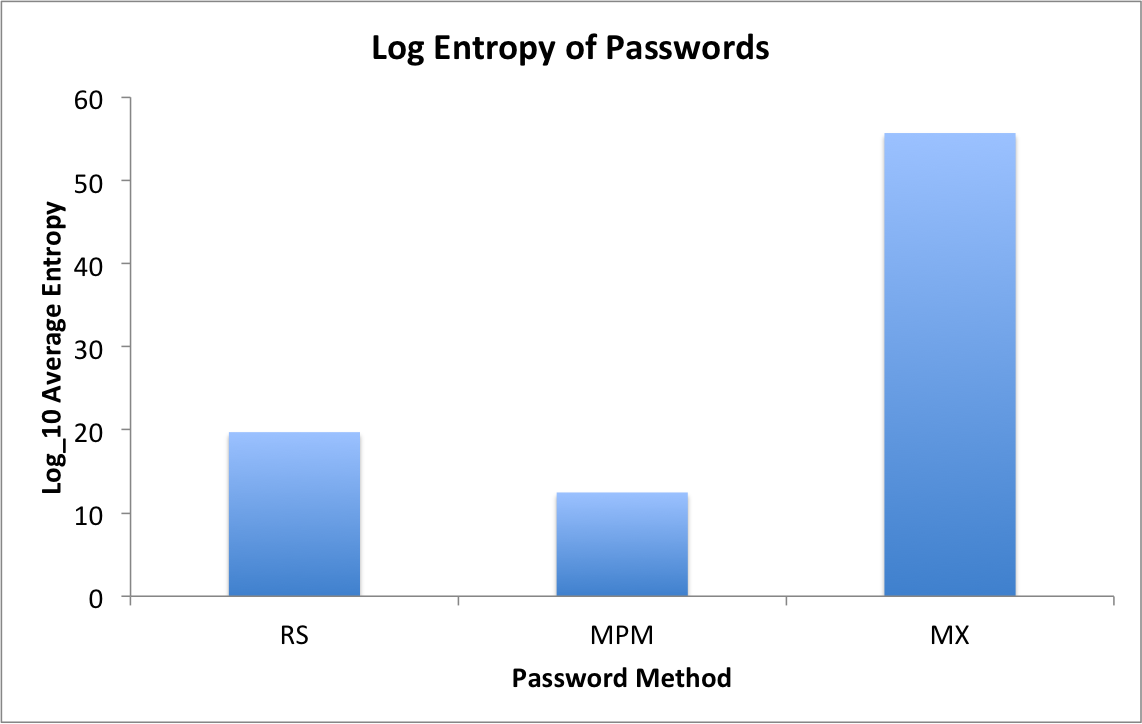
\includegraphics[scale=0.7]{entropy.png}
\caption{Log 10 average entropy of passwords by generation method}
\end{figure}

\begin{table}[h]
\centering
\begin{tabular}{|c|c|c|}
\hline
Password Type & Entropy & $log_{10}$ Entropy \\
\hline
RS & \num{5.4e19}& 19\\
\hline
MPM & \num{4.6e11}& 11\\
\hline
MX & \num{5.7e55}& 56\\
\hline
\end{tabular}
\caption{Average Entropy by password generation method}
\end{table}

\begin{table}[h]
\centering
\begin{tabular}{|c|c|c|c|}
\hline
& RS & MPM & MX \\
\hline
RS & 1 & \num{8.6e-9} & \num{1.1e36} \\
\hline
MPM & \num{1.2e8} & 1 & \num{1.2e44}\\
\hline
MX & \num{9.5e-37}& \num{8.2e-45}& 1 \\
\hline
\end{tabular}
\caption{Entry $(x,y)$ is $\frac{\bar{H_x}}{\bar{H_y}}$ where $\bar{H}$ is average entropy}
\end{table}

\subsection*{MPM Passwords are Woefully Insecure}
\begin{table}
\begin{tabular}{|c|c|c|}
\hline
Mask & User Time (dd:hh:mm:ss) & Passwords Cracked \\
\hline
\texttt{\%l\%l\%l\%l\%d\%d} & 6 & MPM-3,MPM-5 \\
\hline
\texttt{\%l\%l\%l\%l\%d\%d\%d\%d} & 9:33 & MPM-1,MPM-2 \\
\hline
\texttt{\%l\%l\%l\%l\%l\%d\%d} & 2:41 & MPM-6,MPM7\\
\hline
\texttt{\%l\%l\%l\%l\%l\%d\%d\%d\%d} & 5 days (pred.) & - \\
\hline
\texttt{\%a\%a\%a\%a\%a\%a\%a\%a\%a\%a} & $> 10$ years (pred.) & - \\
\hline
\end{tabular}
\caption{Hashcat user time by mask}
\end{table}

\subsection*{RS Passwords and MX Passwords are Secure Against Password Crackers}
It was not possible to use Hashcat's mask attack with RS passwords or MX passwords. The former because Hashcat predicted it would take more than 10 years to search the space, and the latter because Hashcat does not allow masks long enough to represent the MX passwords since searching the space of a mask 20-50 characters long is computationally intractable. Math approximating the feasibility of password cracking on RS and MX passwords was used in lieu of an actual password cracking run. From observing Hashcat running on my system, I have noticed that it generally runs at a speed of between 6.5 million to 7.5 million passwords attempted per second. In order to get a pessimistic lower-bound on the RS and MX passwords, 8 million passwords per second attempted is the speed used in the following calculations. 

\subsubsection*{RS Passwords}
The calculation for the amount of time to search the RS password space with a mask attack is shown below. Note that the number of passwords to search is the same as the entropy for the RS password.

$$\num{5.4e19}~passes \times \frac{sec.}{\num{8.0e6}~passes} \times \frac{year}{\num{3.1e7}~sec.} = \num{2.2e5}~years$$

Thus it would take 220,000 years to search the space of RS passwords with a mask attack using Hashcat on my system.

\subsubsection*{MX Passwords}
Using the same calculation as for the RS passwords yields:
$$\num{5.7e55}~passes \times \frac{sec.}{\num{8.0e6}~passes} \times \frac{year}{\num{3.1e7}~sec.} = \num{2.3e41}~years$$

Thus using a mask attack, it would take \num{2.3e41} years to search the space. This is a period trillions of trillions of ... (etc.) years longer than the age of the universe. While this number certainly excludes the possibility of using a mask attack to break the MX passwords, it is not the most accurate measurement security against a password cracker. This is because the letters in the MX passwords form coherent words, and are thus related to each other. In other words, the letter at position 1 in a password biases what letters could be at position 2. Note that this is not the case for the RS passwords. 

A more appropriate style of attack to attempt to break the MX passwords would be a dictionary attack. Let us make a very generous assumption, and suppose the attacker had a list of all the words that could be put into the passwords (3893) as well as the knowledge that each password would be composed of exactly 5 words. In this scenario, the attacker \emph{does not} know that the passwords follow the pattern described in the methods section of this report. In this case, the entropy is $3893^5$ (there are 3893 options at each of the 5 word-positions in the password). In this case, the entire formula is multiplied by two because there are usually two ways to fix the grammar of an MX password (see methods section):

$$2 \times 3893^5~passes \times \frac{sec.}{\num{8.0e6}~passes} \times \frac{year}{\num{3.1e7}~sec.} = 7,200~years$$

Assuming the attacker new the exact set of words is a very generous assumption, and it would still require 7,200 years for the attacker to search the space with a dictionary attack of the MX passwords. 

Taking this one step further, let us give the attacker one more piece of information. In this case, in addition to knowing the exact set of words, the attacker would also have the words segregated by type of word (i.e. a list of verbs, a list of adjectives, and a list of nouns). We will also give the attacker the knowledge of the structure of the password as adjective noun verb adjective noun. There are 1,466 adjectives; 2,327 nouns; and 100 verbs used to make the MX passwords. Thus, the number of passwords to search is $1466 \times 2327 \times 100 \times 1466 \times 2327 = \num{1.2e15}$:

$$2 \times \num{1.2e15}~passes \times \frac{sec.}{\num{8.0e6}~passes} \times \frac{year}{\num{3.1e7}~sec.} = 9.4~years$$

Even under these extremely generous circumstances, it would still take 9.4 years for an attacker to crack the MX passwords.

\FloatBarrier
\section*{Applications}
This report demonstrates that RS and MX passwords are both acceptably secure against password crackers, but MX passwords are much easier to remember. Websites should not force users to come up with passwords with such draconian rules as ``must contain three of the following: uppercase letter, lowercase letter, number, or digit." Rather, websites should allow users to choose a password consisting of only lowercase letters, as long as this password is long enough. The impetus of change rests with those running websites, rather than with users of websites.

If users were allowed to use MX passwords rather than RS passwords, they would not forget their passwords as easily. Thus, users would be less likely to commit the cardinal sin of computer security of leaving passwords written in plain text on their computer. Furthermore, users wouldn't be so averse to changing their passwords since it is not so challenging to memorize an MX password.
\section*{Conclusion}

\FloatBarrier
\section*{Appendix A: Generated Passwords by Password Type and Participant ID}
\centering
\begin{table}[h]
\begin{tabular}{|m{1.4cm}|m{8cm}|}
\hline
Type-ID & Password \\
\hline
RS-1 & \begin{verbatim} f,K~ym:}7j \end{verbatim} \\
\hline
RS-2 & \begin{verbatim} \fRRWMM>2, \end{verbatim} \\
\hline
RS-3 & \begin{verbatim} T\YJKwj3Ab \end{verbatim} \\
\hline
RS-4 & \begin{verbatim} Mhm@ujAPOZ \end{verbatim} \\
\hline
RS-5 & \begin{verbatim} "?za\HNy\n \end{verbatim} \\
\hline
RS-6 & \begin{verbatim} m!WA,SJBPZ \end{verbatim} \\
\hline
RS-7 & \begin{verbatim} );\U)dn>3^ \end{verbatim} \\
\hline
\end{tabular}
\caption{RS passwords}
\end{table}


\begin{table}[h]
\begin{tabular}{|m{1.4cm}|m{8cm}|}
\hline
Type-ID & Password \\
\hline
MPM-1 & \begin{verbatim} tmwt1988  \end{verbatim} \\
\hline
MPM-2 & \begin{verbatim} hbty1205 \end{verbatim} \\
\hline
MPM-3 & \begin{verbatim} mait10  \end{verbatim} \\
\hline
MPM-4 & \begin{verbatim}  mciagb5722 \end{verbatim} \\
\hline
MPM-5 & \begin{verbatim}  sapf11 \end{verbatim} \\
\hline
MPM-6 & \begin{verbatim} tirwh31 \end{verbatim} \\
\hline
MPM-7 & \begin{verbatim} tcsam16 \end{verbatim} \\
\hline
\end{tabular}
\caption{MPM passwords}
\end{table}

\begin{table}[h]
\begin{tabular}{|m{1.4cm}|m{8cm}|}
\hline
Type-ID & Password \\
\hline
MX-1 & \begin{verbatim} nastyknightschangepoliteanteater  \end{verbatim} \\
\hline
MX-2 & \begin{verbatim} dulldollarshaveshortscience \end{verbatim} \\
\hline
MX-3 & \begin{verbatim} englishrulerunloudwitness  \end{verbatim} \\
\hline
MX-4 & \begin{verbatim} intelligentballoonsharessillyviolin  \end{verbatim} \\
\hline
MX-5 & \begin{verbatim} casualpiebecomesonlyprofit \end{verbatim} \\
\hline
MX-6 & \begin{verbatim} plannedaardvarkdrinksbloodyriverbed \end{verbatim} \\
\hline
MX-7 & \begin{verbatim} unemployedshoemakersignorechangingviolin \end{verbatim} \\
\hline
\end{tabular}
\caption{MX passwords}
\end{table}




\end{document}